\chapter{Referencial Teórico}
\label{cap:ref-teorico}
Neste capítulo estão descritos os fundamentos pertinentes a este trabalho. A Seção \ref{ref-teo:npm} apresenta o conceito e o funcionamento do \gls{npm} bem como a questão das dependências. A Seção \ref{ref-teo:prov_clie} distingue os termos \textit{provedor} e \textit{cliente}. Também para diferenciar termos, a Seção \ref{ref-teo:pac_rel_ver} discorre sobre \textit{pacote}, \textit{release} e \textit{versão}. A Seção \ref{ref-teo:semver} explica o que é \textit{Versionamento Semântico} e o \textit{SemVer} e como eles são utilizados no ecossistema do \gls{npm}. Porfim, a Seção \ref{ref-teo:breaking_change} conceitua e exemplifica as \textit{breaking changes}.

\section{\gls{npm}}
\label{ref-teo:npm}
O \gls{npm} é um gerenciador de pacotes para o \textit{Node.js}. Lançado em 2009, seu principal objetivo é facilitar o compartilhamento de códigos escritos em \textit{Javascript}. Atualmente, o \gls{npm} ocupa a posição de maior repositório para uma dada linguagem, com mais de 1 milhão de projetos\footnote{http://www.modulecounts.com/}. O \gls{npm} permite que, com apenas um simples comando, o usuário realize o download, publique, instale e desinstale pacotes diretamente de vários repositórios. A facilidade proporcionada pelo \gls{npm} corrobora para a grande popularidade do \textit{Javascript} e para que o compartilhamento de bibliotecas seja largamente utilizado, uma vez que 97\% dos aplicativos \textit{web} são oriundos do \textit{NPM}\footnote{https://blog.npmjs.org/post/180868064080/this-year-in-javascript-2018-in-review-and-npms}.

O ecossistema \gls{npm} estimula o compartilhamento de código entre aos pacotes. Por causa disso, dentre os demais repositórios, o \gls{npm} contém a maior distribuição de dependência entre os pacotes \cite{teorical_reference:npm_2}. Dessa maneira, como muitos pacotes estão dependendo mutuamente uns dos outros, há uma gigantesca rede de interconectividade entre os pacotes e, quando há um erro qualquer em algum desses pacotes, um grande número de outros pacotes podem ser afetados. Foi exatamente isso que ocorreu com um pacote chamado \textit{left-pad}\footnote{https://blog.npmjs.org/post/141577284765/kik-left-pad-and-npm}. Esse pacote foi removido do \textit{NPM} por seu desenvolvedor e impactou milhares de pacotes em apenas 2.5 horas, incluindo pacotes renomados como o \textit{babel}\footnote{https://github.com/babel/babel} e o \textit{atom}\footnote{https://github.com/atom/atom} que, devido ao grande número de dependentes, cascatearam o erro para inúmeros outros pacotes.
%In fact, 97\% of the code in a modern web application comes from npm

\section{Provedor e Cliente}
\label{ref-teo:prov_clie}
O pacote provedor é aquele que provê recursos ao pacote cliente, ou seja, contém interfaces públicas para acesso às suas funcionalidades. O termo \textit{pacote provedor} pode ser interpretado como \textit{bibliotecas} ou \textit{dependências}. Por exemplo, quando é executado o seguinte comando

\begin{lstlisting}[style=bash, label=cod:install:provider]
npm install mocha
\end{lstlisting}
o \gls{npm} salva o \textit{mocha} no \textit{package.json} como um provedor. Assim, o pacote \textit{mocha} é um provedor direto, pois foi instalado diretamente pelo usuário. Entretanto, as dependências do \textit{mocha} também são instaladas, mas de forma indireta pelo \gls{npm}. Estes outros pacotes são chamados de \textit{provedores indiretos}, pois não dependem que o usuário instale-os diretamente com o comando \textit{npm install}. A Figura \ref{fig:provider} mostra que, através do comando \textit{npm ls}, o pacote \textit{mocha} é um provedor direto do \textit{client}, pois o \textit{client} requer o \textit{mocha} para executar. Já o pacote \textit{glob} é um provedor direto do \textit{mocha}, e um provedor indireto do pacote \textit{client}.

\begin{figure}
    \centering
    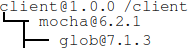
\includegraphics{figuras/provider_directly_undirectly.png}
    \caption{\textit{mocha} como provedor direto e \textit{glob} como indireto do \textit{client}}
    \label{fig:provider}
\end{figure}{}

Já o pacote cliente é aquele que está acessando as interfaces públicas do provedor. Quando uma \textit{break change} é introduzida pelo provedor -- direto ou indireto --, é sempre no pacote cliente que esta \textit{break change} se manifesta, causando o encerramento da execução. O pacote cliente é aquele que possui a responsabilidade de atualizar a versão de seus provedores no \textit{package.json} quando esses publicam uma \textit{release} com correções, enquanto que o pacote provedor possui a responsabilidade de indicar o nível de compatibilidade que sua nova \textit{release} está introduzindo \cite{teorical_reference:semver}.

\section{Pacote, \textit{Release} e Versão}
\label{ref-teo:pac_rel_ver}
Neste trabalho, a palavra \textit{pacote} refere-se a um \textit{software} hospedado no \gls{npm}. Esse \textit{software} contém seu nome, seus arquivos e suas versões. Por exemplo, quando nos referimos ao pacote \textit{mocha}, nos referimos à ideia genérica desse pacote, sem levar em consideração uma versão específica ou seu estado em algum instante, mas sim, apenas ao pacote como um todo.

Já a palavra \textit{release} designa o estado de um pacote em um determinado instante. Uma \textit{release} é denotada por uma versão específica desse pacote, isto é, um conjunto de arquivos distintos das demais \textit{releases}. Cada \textit{release} é acompanhada da publicação de uma nova versão do pacote no \gls{npm}.

Por fim, o termo \textit{versão} é utilizado para especificar e distinguir um determinado estado de uma \textit{release}. Uma \textit{versão} é uma \textit{string} no padrão \textit{SemVer} que identifica unicamente uma determinada \textit{release} e é utilizada pelo \gls{npm} no arquivo \textit{package.json} para especificar um \textit{range} de versões que o cliente aceita.

\section{Versionamento Semântico e \textit{SemVer}}
\label{ref-teo:semver}
O Versionamento Semântico\footnote{https://semver.org} é um padrão para versionamento de \textit{releases} de um projeto que considera o tipo de alteração introduzida na \textit{release}. As regras do Versionamento Semântico foram idealizadas por Tom Preston-Werner -- criador do \textit{GitHub} -- que incentiva todos os desenvolvedores à utilizarem este padrão, uma vez que as regras são baseadas em práticas comuns já utilizadas em projetos \cite{teorical_reference:semver}. Uma \textit{string} de versão no padrão do Versionamento Semântico possui os níveis \textit{<MAJOR>.<MINOR>.<PATCH>}\footnote{a \textit{string} pode ser estendida para versões \textit{beta, alpha, pre}, entre outros, tal como \textit{x.y.z-beta.0}}, que devem ser incrementados, quando o desenvolvedor publicar uma \textit{release}, de acordo com o seguinte critério:

\begin{itemize}
    \item \textit{MAJOR}: deve ser incrementado quando a \textit{release} introduz \textit{breaking changes};
    \item \textit{MINOR}: incrementado quando for adicionado melhorias/novas funcionalidades que mantenham a compatibilidade com as \textit{releases} anteriores; e
    \item \textit{PATCH}: deve ser incrementado quando a \textit{release} contém correção de \textit{bugs}.
\end{itemize}{}

Dessa maneira, se um projeto contém a sua última \textit{release} versionada como \textit{2.1.0}, por exemplo, o seu nível \textit{major} é o 2; o \textit{minor}, 1; e o \textit{patch}, 0. Ao publicar uma nova \textit{release}, se essa conter uma \textit{breaking change}, então deverá ser publicada com a versão \textit{3.0.0}; se for introduzida uma nova funcionalidade, \textit{2.2.0}; se houver uma correção de \textit{bugs}, \textit{2.1.1}.

O \textit{SemVer} é uma \textit{string} de versionamento que especifica um intervalo de versões, ou \textit{range}. Com o \textit{SemVer} é possível especificar quais são as \textit{releases} que o cliente aceita do seu provedor. Há vários padrões de \textit{range}\footnote{https://github.com/npm/node-semver\#ranges} especificados pelo \textit{SemVer}, mas os mais comuns, utilizados pelo \gls{npm}, são:

\begin{itemize}
    \item \textit{X-Ranges (*)}: este \textit{range} especifica para o \gls{npm} que o cliente aceita qualquer nova \textit{release} do provedor, até mesmo as \textit{releases} com \textit{breaking changes};
    \item \textit{Caret Ranges (\textasciicircum)}: este é o \textit{range} mais comum e o padrão do \gls{npm}. Com o \textit{Caret Range}, o cliente especifica que o \gls{npm} só deve descarregar novas \textit{releases} do provedor que contenham novas funcionalidades e correções de erros, mas que não contenham \textit{breaking changes}, ou seja, o cliente aceita todas as \textit{releases} das quais foram atualizadas os níveis \textit{patch} ou \textit{minor};
    \item \textit{Tilde Ranges (\textasciitilde)}: neste \textit{range}, o cliente especifica para o \textit{NPM} que somente as \textit{releases patch} do provedor são aceitas.
\end{itemize}{}

O \gls{npm} utiliza o padrão \textit{SemVer} no arquivo \textit{package.json} -- arquivo de configuração do projeto que contém todas os provedores e suas respectivas versões. Ao executar o comando \textit{npm install express --save}, para instalar o provedor \textit{express}\footnote{https://www.npmjs.com/package/express} por exemplo, o \gls{npm} -- além de descarregar este provedor -- irá salvar no \textit{package.json} o nome do provedor com sua versão atual em modo \textit{range}, de acordo com a Figura \ref{fig:dep_express}.

\begin{figure}
    \centering
    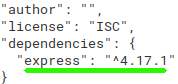
\includegraphics{figuras/dependencies_express.png}
    \caption{Modo como o \gls{npm} salva no \textit{package.json} a versão de uma dependência}
    \label{fig:dep_express}
\end{figure}{}

Com a informação do \textit{range} do provedor no \textit{package.json}, o cliente não precisa se preocupar com as novas atualizações de seus provedores, uma vez que o \gls{npm}, ao instalar novamente os provedores, sempre irá descarregar as \textit{releases} mais recentes que são aceitas pelo \textit{range SemVer}, especificado pelo cliente. Por padrão, o \gls{npm} especifica o \textit{Caret Range}, mas o cliente pode especificar outro \textit{range} manualmente no \textit{package.json} ou pode utilizar a opção \textit{--save-exact} para especificar a versão sem o \textit{range}, fazendo com que o \gls{npm} sempre instale esta versão específica.

\section{Breaking Change}
\label{ref-teo:breaking_change}
Uma \textit{break change} é uma alteração no pacote provedor que produz defeitos nos pacotes clientes \cite{teorical_reference:semver}. As \textit{break changes} surgem quando o pacote provedor, que previamente era executado com sucesso pelo cliente, publica uma \textit{release} que causa no cliente um comportamento inesperado, resultando em um erro. Durante o desenvolvimento de \textit{software}, os provedores precisam introduzir \textit{breaking changes}, pois quando só há \textit{releases} compatíveis com versões anteriores, o \textit{software} perde muitas oportunidades de evolução \cite{teorical_reference:bc_2}. Desta maneira, as \textit{break changes} são importantes para a evolução de um \textit{software}, uma vez que apenas \textit{releases} retro-compatíveis podem estagnar o \textit{software} limitando sua evolução. Assim, as \textit{breaking changes} também são sinônimos de evolução. Exemplo disso é o \textit{Node.js} que publica uma \textit{release} incrementando o nível \textit{major} a cada 6 meses\footnote{https://github.com/nodejs/node\#release-types}. Desta maneira, introduzir \textit{breaking changes} em níveis \textit{major} permite que os \textit{softwares} evoluam sem manter-se preso à versões anteriores.

Para evitar que os impactos de uma \textit{break change} afetem os clientes, os provedores publicam suas \textit{releases} com \textit{breaking changes} incrementando o nível \textit{major} da sua nova versão, seguindo a regra do Versionamento Semântico. Dessa maneira, os clientes de versões prévias que especificaram o provedor com o \textit{range caret} -- \textit{range} especificado por padrão pelo \gls{npm} -- ou o \textit{range tilde} não serão afetados por uma \textit{break change}. Porém, uma \textit{breaking change} pode ser introduzida em uma \textit{release} intencionalmente -- quando é atualizada o nível \textit{major} --, mas também pode ser introduzida inesperadamente -- quando é atualizado os níveis \textit{minor} ou \textit{patch}. Dessa maneira, o problema das \textit{breaking changes} está no fato do desenvolvedor introduzi-las em \textit{releases minor} ou \textit{patch}, resultando em defeitos nos clientes, uma vez que o cliente irá receber essa \textit{release} que contenha \textit{break changes} -- desde que o \textit{range} especificado para a versão do provedor aceite esta \textit{release} --, e se o cliente não espera ou não tratou previamente essa \textit{break change}, com certeza sua execução estará comprometida.

Um exemplo de \textit{breaking change} ocorreu na \textit{release optipng@0.2.0}: a \gls{API} \textit{OptiPng.getBinaryPath} foi renomada para \textit{OptiPng.getBinPath}\footnote{https://github.com/papandreou/node-optipng/pull/6}. Porém, a \gls{API} foi renomeada por engano e a \textit{release} errônea foi publicada em uma versão \textit{minor}, fazendo com que todos os clientes que tinham acesso àquela \gls{API} não a tivesse mais. Assim, o código \ref{cod:bc:optipng} executa normalmente com o \textit{optipng@0.1.1}, mas ao atualizar para o \textit{optipng@0.2.0}, este código sofre uma \textit{breaking change} -- o que não deveria acontecer com uma \textit{release minor}  -- conforme mostra a Figura \ref{fig:bc_optipng} (a).

\begin{lstlisting}[style=Javascript, label=cod:bc:optipng, caption={Código que sofre \textit{breaking change} do \textit{optipng}}]
var OptiPng = require('optipng');
var cb = {apply: () => {}};
OptiPng.getBinaryPath(cb);
\end{lstlisting}

Apesar de ser um erro facilmente detectável, esse foi consertado após 34 dias. E esta correção foi realizada em um \textit{commit}\footnote{https://github.com/papandreou/node-optipng/commit/a155f2b078224be18367847bbcbd3df3c379deea} no qual o desenvolvedor informou no comentário que a renomeação da \gls{API} ocorreu por engano, conforme a Figura \ref{fig:bc_optipng} (b), quando o desenvolvedor desfez a renomeação.

\begin{figure}
    \centering
    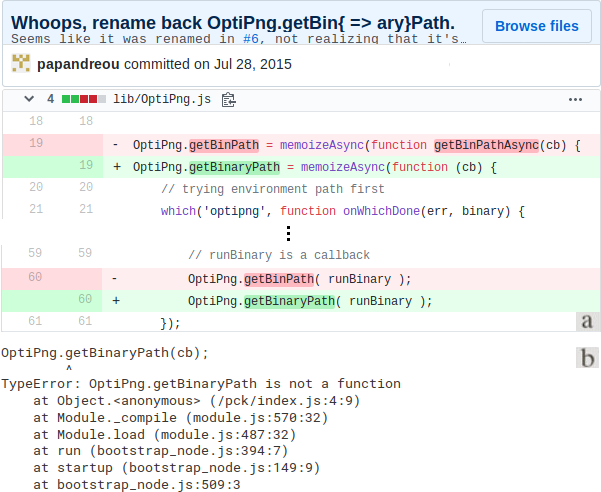
\includegraphics[scale=0.65]{figuras/bc_optipng.png}
    \caption{\textit{a}: \textit{stack trace} da \textit{break change}. \textit{b}: \textit{commit} que corrigiu a \textit{break change}}
    \label{fig:bc_optipng}
\end{figure}{}

\subsection{Casos de \textit{non-break changes}}
Além de alterações que resultam em \textit{breaking changes}, há algumas alterações que são causadas por provedores mas que, nessa pesquisa, não serão consideradas como \textit{breaking changes}. Essas alterações são:

\begin{itemize}
    \item Alterações da versão do \textit{Node.js}: o \textit{Node.js} atualizou o seu nível \textit{major} de \textit{0.x} para \textit{7.x} em apenas 3 anos\footnote{https://nodejs.org/en/download/releases}, mas isso não significa que os pacotes evoluíram seus códigos sempre para a última \textit{release} do \textit{Node.js}, e o inverso é valido, ou seja, os pacotes podem ter evoluído seus códigos na mesma frequência do \textit{Node.js}. Por exemplo, considere um pacote cliente executando no \textit{Node.js 0.x} com um provedor que evoluiu seu código para a sintaxe do \textit{Node.js 6.x}, que não é aceita no \textit{Node.js 0.x}. Desta maneira, não há uma versão do \textit{Node.js}  na qual seja possível executar o pacote cliente sem que no provedor seja manifestado um erro. Assim, erros nos provedores ocasionados por versões do \textit{Node.js} não serão considerados como \textit{break changes}, pois o erro foi causado pelo \textit{Node.js}, que não reconhece a sintaxe, e não pelo provedor;
    \item Exclusão de uma \textit{release}/\textit{provedor} do \gls{npm}: pelas regras do \gls{npm}, uma \textit{release} só pode ser removida até 72 horas após ter sido publicada\footnote{https://docs.npmjs.com/cli/unpublish\#description}. Entretanto, quando uma \textit{release} é removida do \gls{npm} e o cliente especificou aquela \textit{release}, isso gera um erro no \textit{script install}. Assim, o erro é causado pelo \gls{npm} que não consegue encontrar a \textit{release}, e não pelo provedor. No caso do provedor ter sido removido do \gls{npm} o caso é o mesmo: um provedor só pode ser removido após 72 horas. Entretanto, anterior ao acontecimento do \textit{left-pad}, os pacotes -- e \textit{releases} também -- podiam ser removidos do \gls{npm} em qualquer circunstância. Por isso, quando um pacote removido do \gls{npm} causar um erro, não será considerado como uma \textit{break change}.
    \item Alterações em serviços externos: os pacotes podem fazer uso de sistemas externos, tais como acesso à \textit{API}'s de sites e sistemas, e recuperar dados desses. Entretanto, ao longo do tempo, naturalmente, essas \textit{API}'s podem alterar seus dados, o que gera inconsistências em seus clientes. Mas esse tipo de erro não é considerado como uma \textit{break change}; e
    \item Cliente aceita \textit{releases} major do provedor: quando o cliente especifica em seu \textit{package.json} que aceita qualquer \textit{release} do provedor, através de um \textit{X-range}, o cliente então está aceitando \textit{releases} que foram introduzidas \textit{break changes}. Por isso, quando um cliente for impactado por uma \textit{break change} no provedor, e que foi corretamente introduzida em uma \textit{release major}, então o problema está no cliente que aceitou a \textit{break change} mas não a tratou.
\end{itemize}{}

\section{Trabalhos Relacionados}
\label{sec:related_works}